\documentclass[titlepage]{article}

\usepackage[margin=1in]{geometry}
\usepackage{amsmath}
\usepackage{amsfonts}
\usepackage{booktabs}
\usepackage{pgfplots}
\usepackage{enumitem}
\usepackage{placeins}
\usepackage{graphicx}
\usepackage{subcaption}
\usepackage{fancyvrb}
\usepackage{mathtools}

\usetikzlibrary{matrix,chains,positioning,decorations.pathreplacing,arrows}


\author{Eddie Shim}
\title{Coursera Machine Learning Notes}
\date{April 24, 2017}




\begin{document}
	\maketitle
\section{Intro}
\begin{itemize}
	
	\item \textbf{Machine Learning}:
	\\ A subfield of computer science that gives computers ability to learn without being explicitly programmed. Explores the study and construction of algorithms that can learn from and make predictions on data.
	\\
	\item \textbf{Supervised Learning}:
	\\Dataset fed to algorithm includes the dependent variables (answers to problem at hand is part of dataset) \\Eg: regression, classification (predicting housing prices given its characteristics, predicting tumor malignancy); \\(linear regression, logistic regression, neural networks, support vector machines)
	\\
	\item \textbf{Unsupervised Learning}:
	\\Dataset fed to algorithm does not include dependent variables \\Eg: clustering (market segmentation, social networking analysis, facial recognition); \\(k-means, PCA, anomaly detection)
	
	\section{Regression}
	\subsection{Linear Regression}
	For a univariate linear regression, take a dataset of two variables and optimize the linear equation $y= \theta_1 x + \theta_0$. Use the least squares method $\sum_{i=1}^{m} (f(x)-y)^2$, where $(f(x)-y)^2$ represents the residual squared. To minimize residual squared, find $\vec\theta$ which makes the derivative of the cost function equal to 0.
	
	\item \textbf{Cost function for linear regression} (where $\vec{\theta} \in \mathbb{R}^{n+1}$, where $n$ is the number of independent variables):
	\begin{align*}
		J(\vec\theta) &= \frac{1}{2m} \sum_{i=1}^{m}(h_{\theta}(x^{(i)}) - y^{(i)})^2\\
		h_\theta(x) &= \theta_0 + \sum_{i=1}^{n} \theta_i x_i
	\end{align*}
	
	where the framework $h_ \theta$ represents a "hypothesis", or the output prediction of the model
	
	\item \textbf{Gradient descent} (Note: must update all $\theta_j$ simultaneously):
	\begin{align*}
		\theta_j := \theta_j - \alpha \frac{\partial}{\partial \theta_j} J(\vec \theta)
	\end{align*}
	ex: for 2 variable case:
	
	
	\begin{align*}
		\theta_0 &:= \theta_0 - \alpha \frac{1}{m}\sum_{i=1}^{m} (h_\theta(x^{(i)}) - y^{(i)}) \\
		\theta_1 &:= \theta_1 - \alpha \frac{1}{m}\sum_{i=1}^{m} (h_\theta(x^{(i)}) - y^{(i)}) x^{(i)} \\
	\end{align*}
	
	\item \textbf{Feature scaling}: normalizing all independent variables to an appropriate range. Purpose is the speed up gradient descent.
	\begin{align*}
	x_i = \frac{x_i-\mu}{\text{range of } x}
	\end{align*}
	
	\item Note: if $\alpha$ is too large, gradient descent may skip the global minimum point. However, if $\alpha$ is too little, it may take too long to converge.
	
	
	\item \textbf{Normal equation} an alternative to gradient descent:
	\begin{align*}
		\theta = (X^TX)^{-1}y
	\end{align*}

\FloatBarrier
\begin{table} [!htbp]
	\centering
	\begin{tabular}{p{5cm}|p{6cm}}
		\textbf{Gradient Descent} & \textbf{Normal Equation}\\
		\hline
		- need to choose an $\alpha$ & - no need for $\alpha$\\
		- needs many iterations & - no need to iterate, one calculation\\
		- works well even when n is large & - need to compute $(X^TX)^{-1}$ which runs in $O(n^3)$ runtime\\
		& - slow if n is very large
	\end{tabular}
	
	\caption{Pros and Cons}
\end{table}


\item \textbf{Vectorization}: to speed up loops.\\
e.g. Transform the following code from: 

\begin{Verbatim}[obeytabs]
for i = 1:3
   for j = 1:m
      theta(i) := theta(i) - alpha * (1/m)*(h_theta(x(j))-y(j))*x(i);
   end
end
\end{Verbatim}


into:
\begin{verbatim}
theta = theta - alpha * delta;
\end{verbatim}

where $\theta \in \mathbb{R}^{n+1},\ \alpha \in \mathbb{R},\ \delta \in \mathbb{R}^{n+1}$

\subsection{Logistic Regression}
\item A classification algorithm (not really regression, which predicts continuous variable given continuous variable)
\begin{align*}
h_\theta (x) &= g(\theta^Tx), \\
\text{where} \ g(z) &= \frac{1}{1+e^{-z}} \ \ \ (\text{sigmoid function})
\end{align*}

\begin{center}
\begin{tikzpicture}
\begin{axis}[xmin = -4, xmax = 4, ymin = 0, ymax=1, xlabel=$z$,ylabel=$g(z)$]
\addplot[very thick, orange] {1/(1+exp{-x})};
\end{axis}
\end{tikzpicture}	
\end{center}

\item Nice properties:
\begin{itemize} [label = $\bullet$]
	\item {$0 \leq h_\theta (x) \leq 1$}, good for properties of a probability
	\item At $z=0$, $g(z) = 0.5$
	\item Converges to $g(z) =1$ quickly as $g$ increases, and vice versa for 0
	\item We can use these properties to output the probability that an input exists in one of two binary states (1 or 0)
\end{itemize}


\item Terminology: the probability of the output of results equaling 1:
\begin{align*}
h_\theta (x) = p(y=1 | \ x;\theta)
\end{align*}


\item Predict $y=1$ if $\theta^T x \geq 0 \Leftrightarrow \text{if} \ h_\theta(x) = g(\theta^Tx) \geq 0.5$

\item Cost Function:
\begin{align*}
J(\vec\theta) = \frac{1}{m} \sum_{i=1}^{m} \text{cost}(h_\theta (x),y)\\
\end{align*}
where cost $(h_\theta(x),y)$ = 
\[ \begin{cases} 
-log(h_\theta(x)) \ &\text{if} \  y=1\\ 
-log(1-h_\theta(x)) \ &\text{if} \  y =0 
\end{cases} \]


\begin{figure}[h]
	\begin{minipage}{.55\textwidth}
			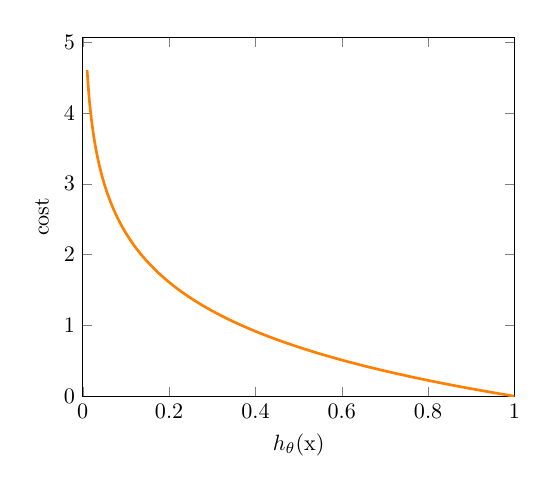
\begin{tikzpicture}[scale=0.8]
			\begin{axis}[xmin=0,xmax=1,ymin=0,xlabel=$h_\theta$(x),ylabel=cost]
			\addplot[very thick,orange, domain=0.01:4.5,smooth,samples=1000] {-ln(x)};
			\end{axis}
			\end{tikzpicture}	
			
	\end{minipage}
		\begin{minipage}{.01\textwidth}
			
			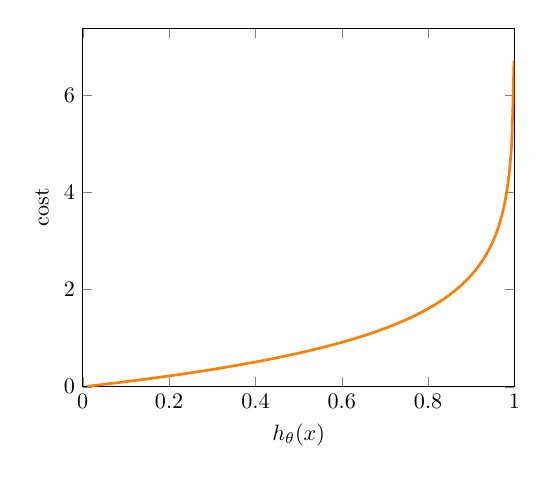
\begin{tikzpicture}[scale=0.8]
			\begin{axis}[xmin=0, xmax=1,xlabel=$h_\theta(x)$,ylabel=cost, ymin=0]
			\addplot[very thick,orange, domain=0.01:4.5,smooth,samples=1000] {-ln(1-x)};
			\end{axis}
			\end{tikzpicture}
			
		\end{minipage}	
		
		\caption{Left: $-log(h_\theta (x))$ ; Right: $-log(1-h_\theta (x))$}
	
	
\end{figure}
\newpage
\item We can create a more succinct function instead of using a piecewise function.\\
\textbf{Cost function for logistic regression}:

\begin{align*} 
\text{cost}(h_\theta(x),y) &= -y*log(h_\theta(x)) - (1-y)*log(1-h_\theta(x))\\
J(\vec{\theta}) &= -\frac{1}{m}\Big(\sum_{i=1}^{m} y^{(i)}*log(h_\theta(x^{(i)})) + (1-y^{(i)})*log(1-h_\theta(x^{(i)}))\Big)
\end{align*}

\subsection{Optimization Algorithms}
\item Given $\theta$, we want to compute 1) $J(\theta)$ and $\frac{\delta}{\delta \theta_j} J(\theta)$ (for $j=0,1,...,n$)
Examples of algorithms we can use to compute the above to motivations include gradient descent, conjugate gradient, BFGS, L-BFGS

\subsection{Regularization}
\item Motivation: to combat overfitting the model, keep certain $\theta_i$ parameters small by taxing $J(\theta)$
\begin{align*}
J(\theta) = \frac{1}{2m} \big[ \sum^{m}_{i=1} (h_\theta (x^{(i)}) - y^{(i)})^2 + \lambda \sum^{n}_{j=1} \theta_j^2 \big]
\end{align*}
where $\lambda$ is the regularization parameter

\item Normal equation with regularization: 
\begin{align*}
\theta = (X^TX + \lambda I)^{-1} X^Ty
\end{align*}

\item Regularized gradient descent:
\begin{align*}
\theta_j := \theta_j - \alpha \big[ \frac{1}{m}\sum^{m}_{i=1} (h_\theta (x^{(i)}) - y^{(i)})x_j^{(i)} + \frac{\lambda}{m} \theta_j \big]
\end{align*}
\section{Neural Networks}

\def\layersep{2.5cm}
\begin{tikzpicture}[shorten >=1pt,->,draw=black!50, node distance=\layersep]
\tikzstyle{every pin edge}=[<-,shorten <=1pt]
\tikzstyle{neuron}=[circle,fill=black!25,minimum size=17pt,inner sep=0pt]
\tikzstyle{input neuron}=[neuron, fill=green!50];
\tikzstyle{output neuron}=[neuron, fill=red!50];
\tikzstyle{hidden neuron}=[neuron, fill=blue!50];
\tikzstyle{annot} = [text width=4em, text centered]

% Draw the input layer nodes
\foreach \name / \y in {1,...,4}
% This is the same as writing \foreach \name / \y in {1/1,2/2,3/3,4/4}
\node[input neuron, pin=left:Input \#\y] (I-\name) at (0,-\y) {};

% Draw the hidden layer nodes
\foreach \name / \y in {1,...,5}
\path[yshift=0.5cm]
node[hidden neuron] (H-\name) at (\layersep,-\y cm) {};

% Draw the output layer node
\node[output neuron,pin={[pin edge={->}]right:Output}, right of=H-3] (O) {};

% Connect every node in the input layer with every node in the
% hidden layer.
\foreach \source in {1,...,4}
\foreach \dest in {1,...,5}
\path (I-\source) edge (H-\dest);

% Connect every node in the hidden layer with the output layer
\foreach \source in {1,...,5}
\path (H-\source) edge (O);

% Annotate the layers
\node[annot,above of=H-1, node distance=1cm] (hl) {Hidden layer};
\node[annot,left of=hl] {Input layer};
\node[annot,right of=hl] {Output layer};
\end{tikzpicture}

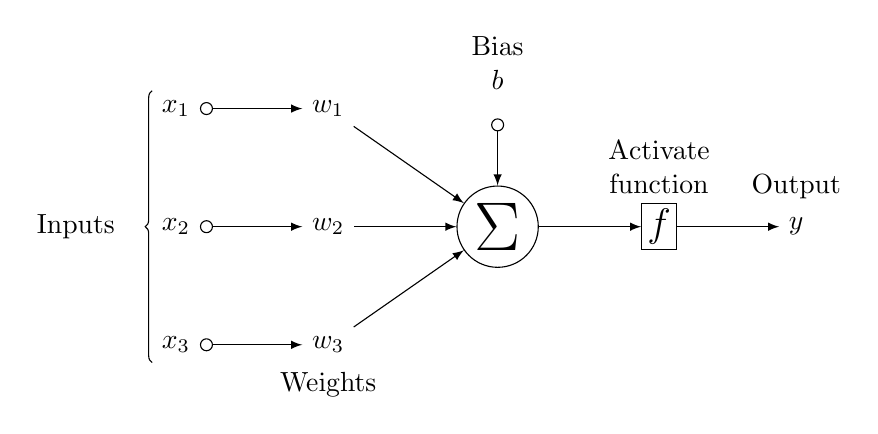
\begin{tikzpicture}[
init/.style={
	draw,
	circle,
	inner sep=2pt,
	font=\Huge,
	join = by -latex
},
squa/.style={
	draw,
	inner sep=2pt,
	font=\Large,
	join = by -latex
},
start chain=2,node distance=13mm
]
\node[on chain=2] 
(x2) {$x_2$};
\node[on chain=2,join=by o-latex] 
{$w_2$};
\node[on chain=2,init] (sigma) 
{$\displaystyle\Sigma$};
\node[on chain=2,squa,label=above:{\parbox{2cm}{\centering Activate \\ function}}]   
{$f$};
\node[on chain=2,label=above:Output,join=by -latex] 
{$y$};
\begin{scope}[start chain=1]
\node[on chain=1] at (0,1.5cm) 
(x1) {$x_1$};
\node[on chain=1,join=by o-latex] 
(w1) {$w_1$};
\end{scope}
\begin{scope}[start chain=3]
\node[on chain=3] at (0,-1.5cm) 
(x3) {$x_3$};
\node[on chain=3,label=below:Weights,join=by o-latex] 
(w3) {$w_3$};
\end{scope}
\node[label=above:\parbox{2cm}{\centering Bias \\ $b$}] at (sigma|-w1) (b) {};

\draw[-latex] (w1) -- (sigma);
\draw[-latex] (w3) -- (sigma);
\draw[o-latex] (b) -- (sigma);

\draw[decorate,decoration={brace,mirror}] (x1.north west) -- node[left=10pt] {Inputs} (x3.south west);
\end{tikzpicture}


\item $a_i ^{(j)}$ refers to the $i^{th}$ node within the $j^{th}$ layer
\item The bias unit is simply =1 and represents a constant within the tuning of $\theta$

\item The network is updated per iteration as such:

\begin{align*}
	&a_1^2{(2)} = g \left(\theta_{10}^{(1)}x_0 + \theta_{11}^{(1)}x_1 + \theta_{12}^{(1)}x_2 + \theta_{13}^{(1)}x_3 \right)\\
	&a_2^2{(2)} = g \left(\theta_{20}^{(1)}x_0 + \theta_{21}^{(1)}x_1 + \theta_{22}^{(1)}x_2 + \theta_{23}^{(1)}x_3 \right)\\
	&a_3^2{(2)} = g \left(\theta_{30}^{(1)}x_0 + \theta_{31}^{(1)}x_1 + \theta_{32}^{(1)}x_2 + \theta_{33}^{(1)}x_3 \right)\\
	h_\theta(x) = &a_1^{(3)} = g \left(\theta_{10}^{(2)}a_0^{(2)} + \theta_{11}^{(2)}a_1^{(2)} + \theta_{12}^{(2)}a_2^{(2)} + 
	\theta_{13}^{(2)}a_3^{(2)} \right)
\end{align*}

\item If network has $s_j$ units in layer $j$, $s_{j+1}$ units in layer $j+1$, then $\theta^{(j)}$ will be of dimension $s_{j+1} *
(s_j+1)$ (ie: $\theta^{j} \in \mathbb{R}^{S_{j+1} \times (S_j + 1)} $)
\\(ex: $\theta^{(1)} \in \mathbb{R}^{3\times 4}$ in above example)

\item To simplify notation, we set the input of the function $g$ as $\vec z$. Thus for example, $a_1^{(2)} = g(z_1^{(2)}), $
\\ where $z_1^{(2)} = \left(\theta_{10}^{(1)}x_0 + \theta_{11}^{(1)}x_1 + \theta_{12}^{(1)}x_2 + \theta_{13}^{(1)}x_3 \right)$

Thus, we can succinctly state:
\begin{align*}
	z_i^{(j+1)} = \theta^{(j)} a^{(j)}\\
	a_i^{(j)} = g(z_i^{(j)}
\end{align*}

\item \textbf{Cost function for Neural Network:}
\begin{align*}
	J(\theta) = -\frac{1}{m} \sum_{i=1}^{m} \sum_{k=1}^{K} \left[y_k^{(i)} log(h_\theta(x^{(i)}))_k + (1-y_k^{(i)})
	log(1-(h_\theta(x^{(i)}))_k)\right] + \frac{\lambda}{2m} \sum_{l=1}^{L-1} \sum_{i=1}^{s_l} \sum_{j=1}^{s_l+1} (\theta _{j,i}^{(l)})^2
\end{align*}

\subsection{Backwards Propagation}
\item \textbf{Motivation:} To calculate the derivate of the cost function. Compare our forwards propagation calibration with the given data $y_i$. We compute a 
$\delta_j^{(l)}$ for every node except our initial layer o $\vec x$, which represents the raw data.

\begin{align*}
\delta_j^{(l)} &= \frac{\partial}{\partial z_j^{(l)}} \text{cost}(i) \\
\text{cost}(i) &= y^{(i)}log h_\theta (x^{(i)}) + (1-y^{(i)}) log h_\theta (x^{(i)})
\end{align*}


\item Example: In a neural network wwith 1 input layer, 1 hidden layer, and 1 output node: \\
$\delta_1^{(3)} = y^{(i)} - a_1^{(3)}$ \\
$\delta_2^{(2)} = \theta_{12}^{(2)} \delta_1^{(3)} + \theta_{22}^{(2)} \delta_2^{(3)}$

\item \textbf{General procedure:}
\begin{enumerate}
\item Given a training set of $\{(x^{(1)}, y^{(1)},...,(x^{(m)}, y^{(m)})\}$
\item Set $\Delta_{ij}^{l} = 0 $ (for all $l,i,j$) \\
\item For $i=1$ to $m$

\begin{itemize} [label = $\bullet$]
	\item Set $a^{(1)} = x^{(i)}$
	\item Perform forward propagation to compute $a^{(l)}$ for $l=2,3,...,L$
	\item Using $y^{(i)}$, compute $\delta^{(L)}=a^{(L)} - y^{(i)}$
	\item Compute $\delta^{(L-1)}, \delta^{(L-2)},...,\delta^{(2)}$
	\item $\Delta_{ij}^{(l)} := \Delta_{ij}^{(l)} + a_j^{(l)}\delta_i^{(l+1)}$
\end{itemize}

\item $\Delta_{ij}^{(l)}:= \frac{1}{m}\Delta_{ij}^{(l)} + \lambda \theta_{ij} ^{(l)}$ if $j \neq 0$
\item $\Delta_{ij}^{(l)}:= \frac{1}{m}\Delta_{ij}^{(l)}$ if $j=0$
\end{enumerate}

\subsection{Gradient Checking}
\item Motivation: an alternate way to calculate the derivative of the cost function, in order to make sure backpropagation is working properly $(\Delta \approx \text{Gradient Approximation})$

\begin{align*}
\frac{\partial}{\partial\theta} J(\theta) &\approx \frac{J(\theta + \epsilon) - J(\theta -\epsilon)}{2\epsilon}\\
\frac{\partial}{\partial\theta_j} J(\theta) &\approx \frac{J(\theta_1,...,\theta_j + \epsilon,...,\theta_n - 
	J(\theta_1,...,\theta_j - \epsilon,...,\theta_n)}{2\epsilon}
\end{align*}

\item Gradient checking is computationally expensive. Backpropagation algorithm is better to use.


\subsection{Neural Network Overview}
\item \textbf{General procedure:}
\begin{enumerate}
\item Randomly initialize weights $\theta \in [-\epsilon, \epsilon]$
\item Implement forward propagation to get $h_\theta(x^{(i)})$ for any $x^{(i)}$
\item Implement code to compute cost function
\item Implement backpropagation to compute partial derivatives $\frac{\partial}{\partial\theta_{jk}^{(l)}} J(\theta)$
\item Use gradient checking to compare $\frac{\partial}{\partial\theta_{jk}^{(l)}} J(\theta)$ computed using backpropagation versus using numerical estimate of gradient of $J(\theta)$. Then disable gradient checking code (one-off check)
\item Use gradient descent or other optimization method with backpropagation to try and minimize $J(\theta)$ as a function of parameters $\theta$. *If $J(\theta)$ is non-convex, then gradient descent may get stuck in a local minima.
\end{enumerate}

\section{Validation/Training}
\item Motivation: prevent over/underfitting the model to the data

\item General ways to trouble shoot errors:
\begin{itemize} [label = $\bullet$]
\item Get more training examples (fixes high variance)
\item Try smaller sets of features (fixes high variance)
\item Try additional features (fixes high bias)
\item Try polynomial features (fixes high bias)
\item Decrease $\lambda$ (fixes high bias)
\item Increase $\lambda$ (fixes high variance)
\end{itemize}

\item \textbf{Misclassification error (0/1) algorithm:}

\begin{align*}
err(h_\theta(x),y) = \begin{cases} 1 &\mbox{if } h_\theta(x) \geq 0.5 \text{ and } y=0 \text{ or } h_\theta < 0.5 \text{ and } y=1 \\
	0 &\mbox{else } \end{cases}
\end{align*}

\begin{align*}
\text{Test Error} = \frac{1}{m_{test}} \sum_{i=1}^{m_{test}} err(h_\theta(x_{test}^{(i)}), y_{test}^{(i)})
\end{align*}

\subsection {Model Selection}
\item \textbf{General procedure:}
\begin{enumerate}
\item \textbf{Training:} Calculate optimal $\theta$ for each polynomial degree using training set (60 \%)
\item \textbf{Cross-Validation:} Using $\theta$ from Step 1, calculate $J(\theta^{(d)}$ for each degree $d$ and choose optimal $d$ using the cross-validation set (20 \%)
\item \textbf{Test:} Estimate Test Error using the test set (20 \%)
\end{enumerate}

\item Plot error over degree of polynomial $d$ for both the training error and CV error in order to visualize fit
\begin{itemize}[label = $\bullet$]
\item Underfit = high bias ($J_{train}(\theta)$ will be high, $J_{CV}(\theta) \approx J_{train}(\theta)$ )
\item Overfit = high variance ($J_{train}(\theta)$ will be low, $J_{CV}(\theta) >> J_{train}(\theta)$ )
\end {itemize}


\item Data Size Impact (Learning Curves)
\begin{itemize} [label= $\bullet$]
	\item If you have high bias (underfit), then increasing datasize will not decrease error an impactful amount
	\item I fyou have high variance (overfit), then more training data helps, as error from cross-validation and training sets converge
\end{itemize}

\section{Large Margin Classification}
\subsection{Support Vector Machines (SVM)}

\item \textbf{Motivation:} A classification algorithm similar to logistic regression, but instead of outputting a probability of a 0 or 1 state, it directly outputs 0 or 1. Classifies by drawing linear decision boundaries.
\begin{align*}
	h_\theta(x) = \begin{cases} 1 &\mbox{if } \theta^Tx \geq 0 \\
		0 &\mbox{else } \end{cases}
\end{align*}


\item \textbf{Cost function for SVM:}
\begin{align*}
	J(\theta) = C \sum_{i}^{m} \left[y^{(i)}cost_1(\theta^Tx^{(i)}) + (1-y^{(i)})cost_0(\theta^Tx^{(i)})\right] + \frac{1}{2} \sum_i^n \theta_j^2
\end{align*}
where $c$ is a weighting constant, similar to the purpose of $\lambda$
\begin{itemize} [label = $\bullet$]
	\item Large $C$: (overfitting) lower bias, high variance (small $\lambda$)
	\item Small $C$: (underfitting) higher bias, low variance (large $\lambda$)
\end{itemize}
\item \textbf{Nice properties of SVM:}
\begin{itemize} [label = $\bullet$]
	\item If $y =1$, we want $\theta^Tx \geq 1$ (not like logistic regression, where $\theta^Tx \geq 0$)
	\item If $y=0$, we want $\theta^Tx \leq -1$ (not like logistic regression, where $\theta^Tx <0$)
\end{itemize}

\begin{figure}[h]
	\begin{minipage}{.55\textwidth}
		\begin{tikzpicture}[scale=0.8]
		\begin{axis}[xmin=-4, xmax= 4, ymin = 0, xlabel = $\theta^Tx$, ylabel = cost]
		\addplot[very thick, orange, domain = -4:1,smooth, samples = 1000] {-(x-1)};
		\addplot[very thick, orange, domain = 1:4,smooth, samples = 1000] {0};
		\end{axis}
		\end{tikzpicture}
		
	\end{minipage}
	\begin{minipage}{.55\textwidth}
		\begin{tikzpicture}[scale=0.8]
		\begin{axis}[xmin=-4, xmax= 4, ymin = 0, xlabel = $\theta^Tx$, ylabel = cost]
		\addplot[very thick, orange, domain = -1:4,smooth, samples = 1000] {x+1};
		\addplot[very thick, orange, domain = -4:-1,smooth, samples = 1000] {0};
		\end{axis}
		\end{tikzpicture}
		
	\end{minipage}
	
	
	\caption{Left:$cost_1(z)$ ; Right: $cost_0(z)$}
	
\end{figure}

\subsection{Kernels}
\item \textbf{Motivation:} A classification algorithm which draws non-linear decision boundaries (features can be polynomials). Kernels are calculated using similarity functions.

\item Example (Gaussian kernel):
\begin{align*}
	f_i = \text{similarity}(x,l^{(i)}) = \text{exp} \left( - \frac{||x-1^{(i)} ||^2}{2\sigma^2} \right) = \text{exp} 
	\left( -  \frac{\sum_{j=1}^{n} (x_j - l_j^{(i)})^2}{2\sigma^2} \right)
\end{align*}

\item Must choose tuning of $\sigma^2.$

\begin{itemize} [label = $\bullet$]
\item Smaller $\sigma^2$: (overfitting) lower bias, higher variance (narrow Gaussian curve)
\item Larger $\sigma^2$: (underfitting) higher bias, lower variance (smoother, flatter Gaussian curve)
\end{itemize}

\item Intuition: calculate the data point $x$'s distance from landmark $l$ (represented by coordinates). Using kernel function $f_i$, determine if $x$ is close/similar enough to $l$ and classify $x$ in binary as $\approx$ 0 or 1.

\item Example: Say you have three landmark points, ${l_1, l_2, l_3}$. To classify data point $x$ as 1 or 0, we plut $x$ into $f_1, f_2, f_3$ to check if $x$ is similar to any locations. Then plug into $\theta_0 + \theta_1f_1 + \theta_2f_2 + \theta3f_3 \geq 0$ to classify $x$ as 1 or 0.

\item General procedure for using SVM with kernels:
\begin{enumerate}
\item Given training set \{$(x^{(1)}, y^{(1)},..,(x^{(m)}, y^{(m)})\}$, set landmarks $l^{(1)} = x^{(1)},...,l^{(m)} = x^{(m)}$
\item $\textbf{(Choice of kernel (sim function)/ choice of } \boldsymbol\sigma^2)$ After choosing which similarity function you will use, calculate feature vector $f^{(i)}$ = $[f_0^{(i)}, f_1^{(i)},...,f_m^{(i)}]'$ for every $x^{(i)}$, where for example $f_1^{(i)} = $ sim$(x^{(i)}, l^{(1)})$
\item $\textbf{(Choice of C, calibration of } \boldsymbol\theta)$ Calibrate weights $\theta \in \Re^{m+1}$ using SVM's cost function, but replacing $\theta^Tx^{(i)}$ with $\theta^T f^{(i)}$
\item For each feature vector from $i=1,...,m$, calculate if $\theta^T f^{(i)} \geq 0, \\$where $\theta^T f^{(i)} = \theta_0 f_0 + \theta_1 f_1 +...+\theta_m f_m$
\end{enumerate}

\item Logistic regression versus SVM:
\begin{itemize} [label = $\bullet$]
\item Let $n$ = number of features ($x \in \Re^{n+1}), m= $ number of training examples.
\item If $n$ is large (relative to $m$), use logistic regression, or SVM without a kernel ("linear kernel") (e.g. $n\geq m, n = 10,000, m = 10...1000)$
\item If $n$ is small, $m$ is intermediate, use SVM with Gaussian kernel (e.g. $n=1...1000, m = 10...10,000)$
\item If $n$ is small, $m$ is large, create/add more features, then use logistic regression or SVM without a kernel (e.g. $n=1...1000, m=50,000+)$
\end{itemize}

\section{Clustering}

\subsection{K-means algorithm}
\item \textbf{Motivation:} Allows for categorization of datapoints $\{x^{(1)},...,x^{(m)}\}$ (unsupervised learning) to an arbitrary cluster group in $k=1,...,K$
\item Essentially an optimization problem trying to minimize distance \\
\item \textbf{General procedure:}
\begin{enumerate}
	\item Given a dataset of $\{x^{(1)},...,x^{(m)}\}$, we want to allocate $K$ number of $\textbf{cluster centroids}$ such that we minimize the total distance between the datasets and cluster centroids.
	\item Randomly allocate the cluster centroids $\{\mu_1,\mu_2,...,\mu_k\}$
	\item (Cluster Assignment) For every $x$ from 1 to $m$, calculate which cluster centroid $k$ is the closest (notated as $c^{(i)} = $ index from $1:k$ corresponding to $x^{(i)}$) where $\boldsymbol{c^{(i)} = \min\limits_{k} || x^{(i)} - \mu_k ||^2}$
	\item (Cluster Movement) Calculate the average of the points assigned to each cluster centroid (example: if datapoints $x^{(1)}, x^{(5)}$ are assigned to cluster centroid $k=3$, then update $\mu_3 = \frac{1}{2} [x^{(1)} + x^{(5)}]$ )
	\item Move each cluster centroid to the previous calculation
	\item Iterate until convergence
\end{enumerate}

\begin{Verbatim} [obeytabs]
while (convergence condition){
for i = 1 to m
c^{(i)} := index (from 1 to K) of cluster centroid closest to x^{(i)}
for k = 1 to K
u_k := average(mean) of points assigned to cluster k
}
\end{Verbatim}

\item \textbf{Choosing number of clusters $K$ (Step 1)}
\begin{itemize}[label = $\bullet$]
	\item No universal/unanimous systematic method yet. Normally people choose by hand by observing visual or function output
	\item (Elbow method): plot cost function $J$ over $K$, (exponentially decreasing function like $\frac{1}{x}$) and pick optimal $K$ (not really rigorous as described by video)
\end{itemize}

\item \textbf{Random initialization (Step 2)}

\begin{itemize} [label=$\bullet$]
	\item Pick $k$ distinct random integers $i_1,...,i_k$ from $\{1,...,m\}$. Then set $\mu_1 = x^{(i_1)},...,\mu_k = x^{(i_k)}$
	\item Code example:
	\begin{Verbatim}[obeytabs]
	for i = 1:100{
	Randomly initialize K-means
	Run K-means. Get c^{(1)},...,c^{(m)}, mu_1,...,mu_K
	Compute cost function (distortion): J(c^{(1)},...,c^{(m)}, mu_1,...,mu_K)
	}
	Pick clustering that gave lowest cost J(c^{(1)},...,c^{(m)}, mu_1,...,mu_K)
	\end{Verbatim}
\end{itemize}

\item\textbf{Optimization objective (Distortion function) (Steps 3 \& 4):}

\begin{align*}
	J(c^{(1)},...,c^{(m)}, \mu_1,...,\mu_K) = \frac{1}{m} \sum_{i=1}^{m} ||x^{(i)} - \mu_{c^{(i)}} ||^2
\end{align*}

\section{Dimensionality Reduction}
\subsection{Principal Component Analysis (PCA)}

\item \textbf{Motivation:} To reduce dataset of $n$ features (unsupervised learning) from $\{x^{(1)},...,x^{(n)}\} \rightarrow \ z^{(1)},...,z^{(k)}\}$, where $x^{(i)} \in \Re^{n}$ and $z^{(i)} \in \Re^{k}$ and $k \leq n$. Allows for data compression (speed and efficiency) and for data visualization.


\item \textbf{Summary of PCA:} Find a lower dimensional surface (represented by $\{u^{(1)},...,u^{(k)}\}$) onto which to project the data, so as to minimize the squared projection error. Features with high correlation can be represented in lower dimensions while maintaining original data variance.

\item *Not the same as linear regression, which minimizes distance between line of best fit and data (vertical). In PCA, you minimize orthogonal distances from the line of best fit and data (angled). We want to minimize the following equation which represents the distance between the data and the principal component:

\begin{align*}
	\frac{1}{m} \sum_{i=1}^{m} ||x^{(i)} - x_{approx}^{(i)} ||^2
\end{align*}

\item \textbf{General procedure:}
\begin{enumerate}
	\item Take data and mean normalize it (calculate $\mu_j = \frac{1}{m}\sum_{i=1}^m x_j^{(i)}$ and replace each $x_j^{(i)}$ with $x_j - \mu_j$ as the data). Optimally, feature scale the data as well.
	\item Compute covariance matrix:
	\begin{align*}
		\Sigma = \frac{1}{m} \sum_{i=1}{n} (x^{(i)})(x^{(i)})^T
	\end{align*}
	\item Compute eigenvectors of matrix $\Sigma$:
	\begin{verbatim}
	[U,S,V] = svd(Sigma)
	\end{verbatim}
	Where svd is the singular value decomposition algorithm and $U = [u^{(1)}, u^{(2)},....,u^{(n)}] \in \Re^{n \times n}$
	\item Take the first $k$ columns of $U$, defined as matrix $U_{reduced} = [u^{(1)}, u^{(2)},..., u^{(k)}]$.
	Calculate our desired result $z = U_{reduced}^T x$, where $z \in \Re^k$.
\end{enumerate}

\item \textbf{(Choosing $k$/ testing quality of PCA)} We want to preserve variance in the original data, up to (1-$\alpha$) \%. Thus we choose $k$ to be the smallest value such that

\begin{align*}
	\frac{\text{average squared projection error}}{\text{total variation in the data}} = \frac{ \frac{1}{m}
		\sum_{i=1}^{m} || x^{(i)} - x_{approx}^{(i)}||^2}{\frac{1}{m}\sum_{i=1}^{m}||x^{(i)}||^2} = 1 - 
	\frac{\sum_{i=1}^k S_{ii}}{\sum_{i=1}^{n} S_{ii}} \leq \alpha
\end{align*}
Where $SS_{ii} \in \Re^{n\times n}$ is a diagonal matrix given by a singular value decomposition. Of the two formulas which represent variance retention, the second is more computationally efficient in finding the optimal $k$.

\section{Anomaly Detection}
\item \textbf{Motivation:} Allows for identification of outliers/anomalies. Used for unsupervised learning, but aspects of it still draws from supervised learning concepts. (ex: QA testing on aircraft engines, financial fraud detection, monitoring computers in data center)
\item \textbf{General procedure (Gaussian distribution example):}
\begin{enumerate}
	\item Choose features $x_i$ which might be indicative of anomalous examples
	\item Fit parameters $\mu_1,...,\mu_n, \sigma_1^2,...,\sigma_n^2$, where:
	\begin{align*}
		\mu_j &= \frac{1}{m} \sum_{i=1}^{m} x_j^{(i)}\\
		\sigma_j^2 &= \frac{1}{m} \sum_{i=1}^{m} (x_j^{(i)} -\mu_j)^2
	\end{align*}
	\item Given new example $x$, compute $p(x)$, where:
	\begin{align*}
		p(x) = \prod_{j=1}^n p(x_j; \mu_j, \sigma_j^2) = \prod_{j=1}^n \frac{1}{\sqrt{2\pi}\sigma_j}
		exp(-\frac{(x_j-\mu_j)^2}{2\sigma_j^2})
	\end{align*}
	\item Define $x$ as an anomaly if $p(x) < \epsilon$ (set $y=1$), and $x$ as normal if $p(x) \geq \epsilon$ (set $y=0$)
\end{enumerate}

\item Anomaly detection vs. supervised learning:
\begin{table} [h]
	\centering
	\begin{tabular}{p{8cm}|p{8cm}}
		
		\textbf{Anomaly Detection} & \textbf{Supervised Learning (e.g. logistic regression)}\\
		\hline
		- Very small number of positive examples ($y=1$). 0-20 is common. Large number of negative examples ($y=0$) & - Large number of positive and negative examples \\
		- Many different types of anomalies. Hard for any algorithm to learn from positive examples what the anomalies look like; future anomalies may look nothing like any of the anomalous examples we've seen so far & - Enough positive examples for algorithm to get a sense of what positive examples are like, future positive examples likely to be similar to ones in training set\\
		- e.g.: fraud detection, manufacturing, monitoring machines in data center & - e.g.: email spam classification, weather prediciton, cancer classification\\
		
	\end{tabular}
\end{table}

\item \textbf{Multivariate Gaussian Distribution:} Allows for skewing of normal curve in order to capture correlated data (e.g.: changing top-down views of 2-d graphs from circles into ellipses by chaging off diagonals of $\Sigma$)

\begin{align*}
	p(x;\mu,\Sigma) &= \frac{1}{(2\pi)^{\frac{n}{2}} | \Sigma|^{\frac{1}{2}}} exp \left(-\frac{1}{2}
	(x-\mu)^T\Sigma^{-1} (x-\mu) \right)\\
	\mu_j&= \frac{1}{m} \sum_{i=1}^m x^{(i)}\\
	\Sigma &= \frac{1}{m} \sum_{i=1}^m (x^{(i)}-\mu_j)(x^{(i)}-\mu_j)^T
\end{align*}

where $\mu \in \Re^n$ and $\Sigma \in \Re^{n \times n}$ (covariance matrix)

\item Cons of using multivariate Gaussian: computationally more expensive, must have $m>n$ in order for $\Sigma$ to be invertible, can manually capture correlations in univariate Gaussian by engineering extra features (e.g.: $x_3 = \frac{x_1}{x_2})$)

\section{Recommender Systems}
\item Examples: Netflix's movie recommender, Amazon's product recommender
\subsection{Collaborative Filtering}
\item Essentially a linear regression problem, using regularized gradient descent to find optimal $\vec x$ and $\vec \theta$
\item \textbf{Problem formulation:}
\begin{itemize}[label = $\bullet$]
	\item $\theta^{(j)}$ = parameter vector for user $j$ (calibrated weights for a user's category preferences)
	\item $x^{(i)}$ = feature vector for movie $i$ (calibrated weights for categorization of movie)
	\item $r(i,j) =1$ if user $j$ has rated movie $i$ (0 otherwise)
	\item $y^{(i,j)}$ = rating by user $j$ on movie $i$ (if defined)
	%\item For user $j$, movie $i$, predicted rating = $(\theta^{(j)}^T(x^{(i)}))$
	\item $n_m$ = number of movies
	\item $n_u$ = number of users
\end{itemize}

\textbf{General procedure:}
\begin{enumerate}
	\item Initialize $x^{(1)},...,x^{(n_m)}, \theta^{(1)},...,\theta^{(n_m)}$ to small random values (similar to neural network to ensure gradient descent starts at different values)
	\item Minimize $J(x^{(1)},...,x^{(n_m)}, \theta^{(1)},...,\theta^{(n_m)}$ using gradient descent (or another optimization algorithm). For every $j=1,...,n_u, i=1,...,n_m$:
	\begin{align*}
		x_k^{(i)} &:= x_k^{(i)} - \alpha \left( \sum_{j:r(i,j)=1} ((\theta^{(j)})^T x^{(i)} - y^{(i,j)}) \theta^{(j)} + \lambda x_k^{(i)}\right)\\
		\theta_k^{(j)} &:= \theta_K^{(j)} - \alpha \left( \sum_{i:r(i,j)=1} ((\theta^{(j)})^T x^{(i)} - y^{(i,j)})x^{(i)} + \lambda \theta^{(j)}\right)
	\end{align*}
	\item For a user with parameters $\theta$ and a product with learned features $x$, predict a rating of $\theta^Tx$
\end{enumerate}

\section{Dealing with Large Data}
\subsection{Stochastic Gradient Descent}

\item In batch gradient descent, can be computationally expensive to calculate $\theta_j$:
\begin{align*}
	\theta_j := \theta_j - \alpha \frac{1}{m} \sum_{i=1}^{m} (h_\theta (x^{(i)} - y^{(i)}))x_j^{(i)}
\end{align*}

because as the size of the dataset $m$ grows, the computation must loop $m$ times in order to take one step.

\item \textbf{General procedure for stochastic gradient descent:}
\begin{enumerate}
	\item Randomly shuffle dataset
	\item Run gradient descent on loop which updates per data $x^{(i)}$ instead of entire dataset of size $m$ at once:
	\begin{Verbatim}[obeytabs]
	repeat{
	for i:=1,...,m{
	\theta_j:= \theta - \alpha(h_theta(x^{(i)}) - y^{(i)})x_j^{(i)}
	(for every j = 0,...,n)
	}
	}
	\end{Verbatim}
	\item Plot $J(\theta)$ over number of iterations to check how well $\theta$ is being tuned (cost is decreasing over time and converging)
	\item Tune learning rate $\alpha$ as needed. Decrease $\alpha$ in order to help $\theta$ converge, if the cost seems divergent
	\end{enumerate}
	
	\item The difference: batch gradient descent requires $m$ calculations to travel one step. Stochastic gradient descent takes one step per iteration, taking $m$ steps by the time it loops through $1:m$. Usually requires anywhere from one to ten times $m$ of calculations to converge.
	
	\item Cost function is not necessarily monotonically decreasing, can bounce around
	
	\subsection{Mini-Batch Gradient Descent}
	\item Can be faster than stochastic gradient descent. Instead of looking updating per one example of data, mini-batch descent udpates per $b$ examples of data
	\item \textbf{General procedure} (example when $b=10$):
	\begin{enumerate}
	\item Set batch size $b$ (e.g. say $b = 10$, on a dataset of $m=1000$)
	\item Run gradient descent on loop which updates per $b$ batches of data $x^{(i)}$\\
	for $i = 1,11,21,31,...,991$
	\begin{align*}
	\theta_j := \theta_j - \alpha \frac{1}{10} \sum_{k=i}^{i+9} (h_\theta (x^{(k)} - y^{(k)}))x_j^{(k)}
	\end{align*}
	\end{enumerate}
	
	\end{itemize}
	\end{document}
